\documentclass{AIAA}
\usepackage{amsfonts,amsmath,amssymb}
\usepackage{graphicx}
\usepackage{color}
\usepackage{url}
\usepackage{hyperref}
\begin{document}
\title{A New Actuator for On-Orbit Inspection}
\author{Benjamin Z. Reinhardt \footnote{Sibley School of Mechanical and Aerospace Engineering, bzr3@cornell.edu, and AIAA Student Member} and Mason A. Peck \footnote{Associate Professor, Sibley School of Mechanical and Aerospace Engineering, Full Member}}
\affiliation{Cornell University, Ithaca, NY, 14850}
%Changelog:
%8/7/2014 - bzr3 - Uploaded for editing 

%note, if it throws a 
%\begin{abstract}
%Phenomena such as electromagnetic forces scale with linear dimensions in ways that make small spacecraft qualitatively different from larger ones.  Specifically, small scale may be capable of a new kind of mission architecture, inspecting and servicing larger spacecraft in close proximity without mechanical contact. Nearly all current technologies for applying force and torque between two spacecraft share a disadvantage: they require either propellant or mechanical contact. By using the force between a magnetic field and the electric currents it induces in a conductive target, a new technology known as an induction coupler exploits eddy-current effects to control the relative position and orientation between a chaser spacecraft and a target without mechanical contact. The induction coupler does not rely on familiar magnetic attraction and repulsion, which would require ferromagnetic materials on the target.  In contrast, and induction coupler is broadly applicable for even uncooperative targets, as long as the target includes conductive materials, as is generally the case for spacecraft.  This paper presents an overview of an induction coupler system, outlines design requirements through a case study of an inspection mission relevant to the International Space Station, and establishes the feasibility of flight applications through a description of ongoing experimental work.
%\end{abstract}
\begin{abstract}
Induction couplers are a new technology for controlling the relative position and orientation between a chaser spacecraft and a target without mechanical contact. Induction couplers exploit eddy-current effects to produce force and torque relative to a conductive target without relying on magnetic dipole interactions or cooperation from the target. This paper presents an overview of an induction coupler system, outlines design requirements through a case study of an inspection mission relevant to the International Space Station, and establishes the feasibility of flight applications through a description of ongoing experimental work.
\end{abstract}
 

\maketitle

\section*{Nomenclature}
%%(Nomenclature entries should have the units identified)\\
\noindent\begin{tabular}{@{}lcl@{}}
\textbf{B}  &=& Magnetic Field \\
\textbf{A}&=&    Magnetic Vector Potential \\
$\mu_0$&=& Permeability of Free Space \\
$\sigma$ &=& Conductivity of target material \\
$\hat{\textbf{n}}$ &=& Vector normal to surface \\
$\hat{\textbf{a}}$   &=& Spin axis direction\\
\textbf{d} &=& Induction coupler position in body frame \\
$\omega$ &=& Angular velocity \\
$\beta$ &=& Thrust Ratio \\
C &=& Scaling factor from magnet properties \\
g   &=& Gap between plate and induction coupler \\
b  &=& Conductive surface thickness \\
$r_O$  &=& Induction coupler outer radius \\
$r_i$  &=& Induction coupler inner radius \\
m  &=& Inspector mass \\
I &=& Inspector inertia \\
J &=& Input Jacobian \\
\end{tabular} \\

\section{Introduction} 

%% TODO - repeated whole cloth from the abstract should it be like that
Nearly all current technologies for applying force and torque between two spacecraft share a disadvantage: they require either propellant or mechanical contact. By using the force between a magnetic field and the electric currents it induces in a conductive target, a new technology known as an induction coupler exploits eddy-current effects to control the relative position and orientation between a chaser spacecraft and a target without mechanical contact. The induction coupler does not rely on familiar magnetic attraction and repulsion, which would require ferromagnetic materials on the target.  In contrast, and induction coupler is broadly applicable for even uncooperative targets, as long as the target includes conductive materials, as is generally the case for spacecraft.

An induction coupler creates actuation force by producing a time-varying magnetic field that induces eddy-currents  through the conductive materials in a target. The coupler's magnetic field then exerts a force on these currents and thus the target. The coupler requires no mechanical contact with a target, nor does it demand cooperation from the target. The coupler operates on electricity alone, enabling close-proximity navigation without propellant. Because most satellites include conductive material in their structure-notably aluminum honeycomb with aluminum facesheets, aluminum isogrid, and aluminum truss elements-induction couplers may be the closest thing we have to science fiction's tractor beam: a device that can produce contactless force on an uncooperative target. It can also be thought of as a contactless momentum-transfer actuator.

Induction couplers show promise for spaceflight applications, offering three major advantages. First, the force associated with magnetic fields across meter-scale distances can dominate gravity, aerodynamic drag, and other effects, which are far less pronounced in orbit than in a terrestrial environment. Second, fully deployed spacecraft are fragile and rarely offer straightforward means for mechanical grappling; so, the ability to interact without the potential for contact damage is valuable. Third, induction couplers offer the ability to maneuver without propellant, eliminating risks associated with thruster-plume impingement \cite{BaerwaldR.S.1977}
and extending the useable lifetime of the chaser spacecraft.
A small spacecraft could use induction couplers to control its motion relative to a much larger target like the International Space Station (ISS), crawling just above the target's surface without ever touching. This on-orbit inspection technique resembles the operations concept for underwater robots that now inspect pipelines and shipwrecks. \cite{Whitcomb2000}

%Ben: I'm pretty sure this is unecessary
%\begin{figure}
%\includegraphics[width = 6cm, height = 6cm %{figures/Induction_Coupler_Overview_Diagram.jpg}
%\label{fig:inspector_diagram}
%\caption{A spacecraft can use an induction coupler with three spinning magnets to create actuation force and torque}
%\end{figure}
 
Current interest in on-orbit servicing (OOS) is a strong motivation for advancing induction coupler technology. \cite{Ambrose2012}
 One of the more compelling use cases is that of a small inspection vehicle whose interactions with the target do not produce significant motion in that target-for example, an ISS inspection vehicle. Such a vehicle is primarily concerned with regulating planar motion along the surface of the target and stabilization of out-of-plane translation. This paper describes a study of how the in-plane component of that motion can be achieved with induction couplers.



\section{Background}
\subsection{Other Technologies}

There are other technologies that can produce contactless forces between a spacecraft and a target. Coulomb force has been shown to produce useful interactions between two charged spacecraft as long as the distance between them is less than the Debye length. \cite{coulombtether} A number of different systems produce contactless forces with magnetic interactions among controlled dipoles on both the spacecraft and the target.\cite{dipoleplanning} \cite{Kong2004}
All such approaches place requirements for specific hardware on both the chaser and the target (that is, the target must have launched with certain features already in place.) Implementing these systems is not standard practice, and in fact no spacecraft currently in orbit are known to include components designed for contactless grappling through such techniques.

Laser tweezers can produce contactless force on an uncooperative target. \cite{lasertweezers}However, the tweezers are best at manipulating micron- scale particles, a size restriction that no spacecraft beyond Technology Readiness Level (TRL) $1$ can meet. \cite{lasermirrors} Thruster plumes can also produce forces between a chaser and a target. However, typically the combustion products from thrusters carry significant risk of contaminating optical instruments and solar panels, among other disadvantages. We conclude that current technology is limited to direct mechanical contact as the only general solution for manipulating a target that has not been designed to be cooperative.  This limitation motivates the present study.

\subsection{Induced Current Force}

Eddy-current force starts with a time-varying magnetic field. The field induces an electrical eddy current in any conductive material nearby. In turn, that induced current interacts with the original magnetic field, producing force between the conductive material and the source of the magnetic field.

The currents in the conductor depend on the geometry of the target, its conductivity, $\sigma$, the direction and magnitude of both \textbf{B} and $\frac{d\textbf{B}}{dt}$, and the velocity and position of the induction coupler relative to the target. Compounding the subtlety is the unavoidable coupling between the magnetic field and the kinematics of the magnets in the induction coupler. These interdependencies make the force sensitive to the state of the system. Induction couplers exhibit many nonlinearities, which demand a rigorous and informed approach to implementing the technology.

Eddy-current force is a consequence of Maxwell's equations:

\begin{equation}\label{eq:FaradayInduction}
\nabla \times \textbf{E} = -\frac{d\textbf{B}}{dt}
\end{equation}
\begin{equation}\label{eq:AmperesLaw}
\nabla \times \textbf{B} = \mu_0 \textbf{J}
\end{equation}
\begin{equation}\label{eq:GaussLaw}
\nabla \cdot \textbf{B} = 0
\end{equation}
Any material with finite conductivity experiences a voltage gradient in response to a time-varying magnetic field. 
\begin{equation}\label{eq:currentflow}
\textbf{J}=\sigma \textbf{E}
\end{equation}

The voltage difference induces a current in the material that in turn generates its own magnetic field. The resulting field has a vector potential that obeys 
\begin{equation}\label{eq:vectorPotential}
\textbf{B} = \nabla \times \textbf{A}
\end{equation}
\begin{equation} \label{eq:Efield}
\textbf{E} =  -\frac{d\textbf{A}}{dt} - \nabla V
\end{equation}

If the conductive plate is linear and simply connected, the governing equations can be combined into a partial differential equation describing the propagation of $\textbf{A}$ through the plate \cite{Smyth1989}

\begin{equation}\label{eq:governingPDE}
\nabla^2 \textbf{A} = \mu_0\sigma \frac{d\textbf{A}}{dt}
\end{equation}
Once \textbf{A} is known on the surface of the plate, Maxwell's stress tensor solves for the force between the plate and the magnetic source. Because there is no electric field exterior to the plate, Maxwell's stress tensor ($\overset{\leftrightarrow  }{ \mathbf{\sigma} }$) reduces to
\begin{equation} \label{eq:stressTensor}
\overset{\leftrightarrow  }{ \mathbf{\sigma} } = \frac{1}{\mu_0} \left[ \mathbf{B}\otimes\mathbf{B} - \frac{B^2 }{2} (\mathbf{\hat x}\otimes\mathbf{\hat x} + \mathbf{\hat y}\otimes\mathbf{\hat y} + \mathbf{\hat z}\otimes\mathbf{\hat z}) \right]
\end{equation}

%" src="//upload.wikimedia.org/math/8/d/e/8dea2b36115634afa876918c145f67bf.png">

% TODO Update this figure - make the vectors correct, perhaps make isometric
\begin{figure}
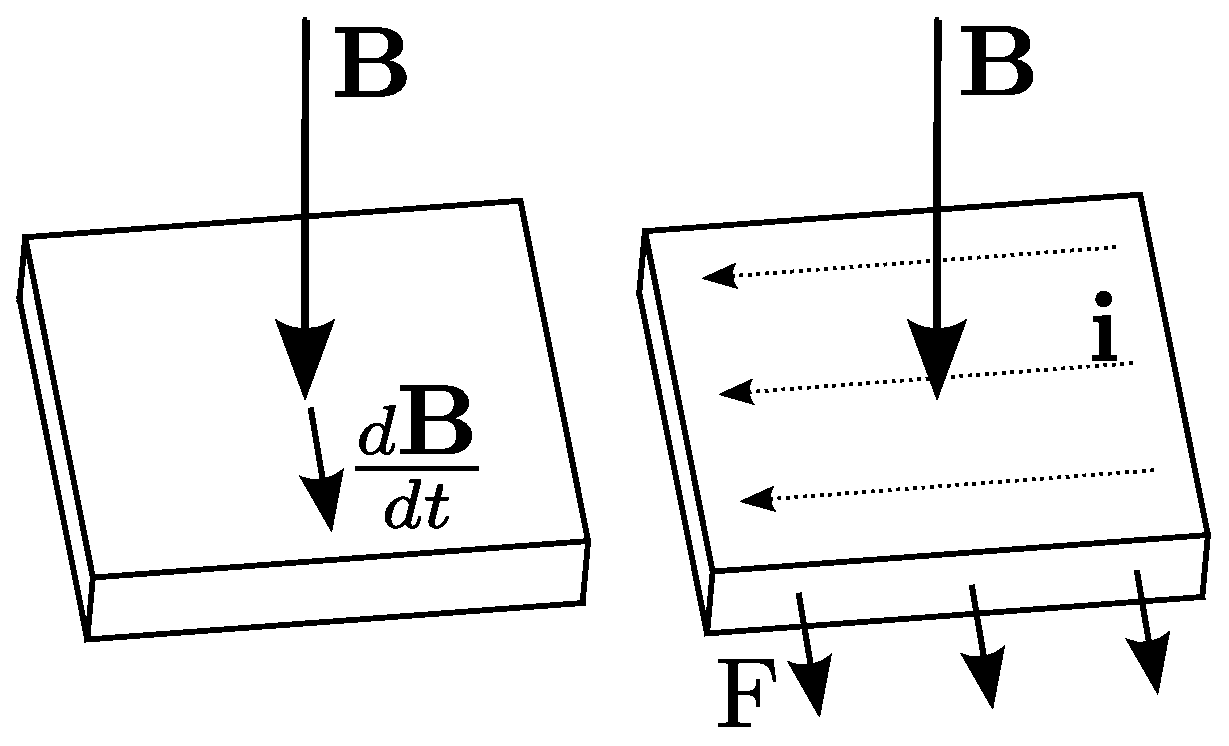
\includegraphics[width = 6cm, height = 6cm ]{figures/iso_force_creation.eps}
\label{fig:force_generation}
\caption{Creating graphical intuition for the problem - a magnetic field directed into the conductor changes in the upward direction. This change induces a current to the left that interact with the original B field to create a downward force.}
\end{figure}

There are many ways to find the magnetic potential in the plate and its resultant actuation force, but few of them are suitable for a model that includes feedback control and rigid-body dynamics. \cite{Paudel2013}
Finite element methods are the standard approach to solving this class of problems quasistatically. However, even those few commercially available FEM packages that can account for a moving source field are computationally expensive and require hand-tuning for each new geometries. These drawbacks make them unsuitable for the dynamical simulations necessary for online control. 

There are also several analytical models for eddy-current forces, but most are also unsuitable for dynamical systems. Most of these models do not take into account a moving source field, which is an essential part of a dynamic system. All analytical solutions to the partial differential equation describing eddy-current propagation are tied to specific geometries. This is not inherently a problem, but most of the assumptions about the orientation of the field are too restrictive to be useful in a dynamic system that can move in 6 DoF near the conductive surface. 

Paudel and Bird introduced an analytical model that both relaxes the geometry restrictions and accounts for a moving magnetic source. Their method finds transient force between a time-varying, moving magnetic source field and a large flat conductive plate. \cite{Paudel2012t}
This model can also be simplified to a computationally-lightweight steady-state solution that finds the force from a magnetic field with a single frequency component. \cite{Paudel2012ss}
The steady-state model is a good approximation when 
\begin{enumerate}
\item There are no interactions between the fields of multiple magnet arrays. 
\item The mechanical frequencies are much lower than the propagation speed of the magnetic field through the conductor.
\item The changing magnetic field has only one frequency component.
\end{enumerate}
This paper uses the steady-state Paudel and Bird method to model the force from the spinning magnet arrays in an induction coupler. 
 
%% TODO THIS PARAGRAPH NEEDS TO BE TRUTHIFIED
Systems of induction couplers can produce force in any direction relative to the target, for example both tangential and perpendicular to a surface on that target. Therefore, a chaser spacecraft generating a time-varying magnetic field can produce forces in all three translational degrees of freedom. Two induction couplers separated by a moment arm can also produce torques, for complete 6DoF actuation.
%% TODO - move this. Perhaps include figures for this. 
There are two ways for an induction coupler to generate its changing magnetic fields and resultant force: permanent magnets that move mechanically and electromagnets driven by time-varying currents. Each type of magnet is especially good at producing forces in different directions. For example, a single electromagnet with a sinusoidal driving current always repels the target. \cite{Reinhardt2012}.  A rotating permanent magnet is effective in producing a shear force, i.e. a force that lies in the plane of a surface.  Replicating the pure repulsive force of an electromagnet with a permanent magnet would require either a linear actuator or a complicated set of linkages. Therefore, a spacecraft that implements induction couplers likely incorporates a combination of permanent magnets and electromagnets..  This paper focuses primarily on a free-flyer inspection vehicle which uses those shear forces to move along its target. 


\section{Mission Description}
\label{sec:mission}
An inspector spacecraft with induction couplers can fulfill a number of functions including verifying the state of health, performing mechanical tasks, or providing communications and other logistical support for astronauts during extravehicular activity (EVA). It may be possible for the eddy currents use for locomotion to detect mechanical damage, as is currently done on some aircraft. \cite{Yang2010}
 This paper focuses on the International Space Station (ISS), but a similar inspection spacecraft could enable unique OOS missions to inspect and repair other large satellites.

The inspection spacecraft described here uses induction couplers to pull itself along the aluminum exterior of the ISS, maintaining a separation distance of a few centimeters. In doing so, it acts like a damage-inspection Roomba,\cite{Tribelhorn2007}
 canvassing the surface and automatically detecting damage from micrometeorite strikes. An alternative operations concept is one in which the inspector is controlled directly by an astronaut to evaluate some region of interest and possibly use an attached robotic arm to effect a repair. In yet another concept, the spacecraft acts like an extra pair of hands during an EVA, remaining near an astronaut and holding tools. NASA's Robonaut and the Mobile Servicing System (the Canadian robotic arm on ISS) have demonstrated the value of such a capability but are limited by rails to specific locations. \cite{Ambrose2012}
The ability to traverse the exterior of the ISS without being constrained to travel on rails, attach to specific hard points, or manage a finite propellant supply can free up one of the most valuable resources on the ISS, astronaut time, and may augment astronaut safety.

\begin{figure}
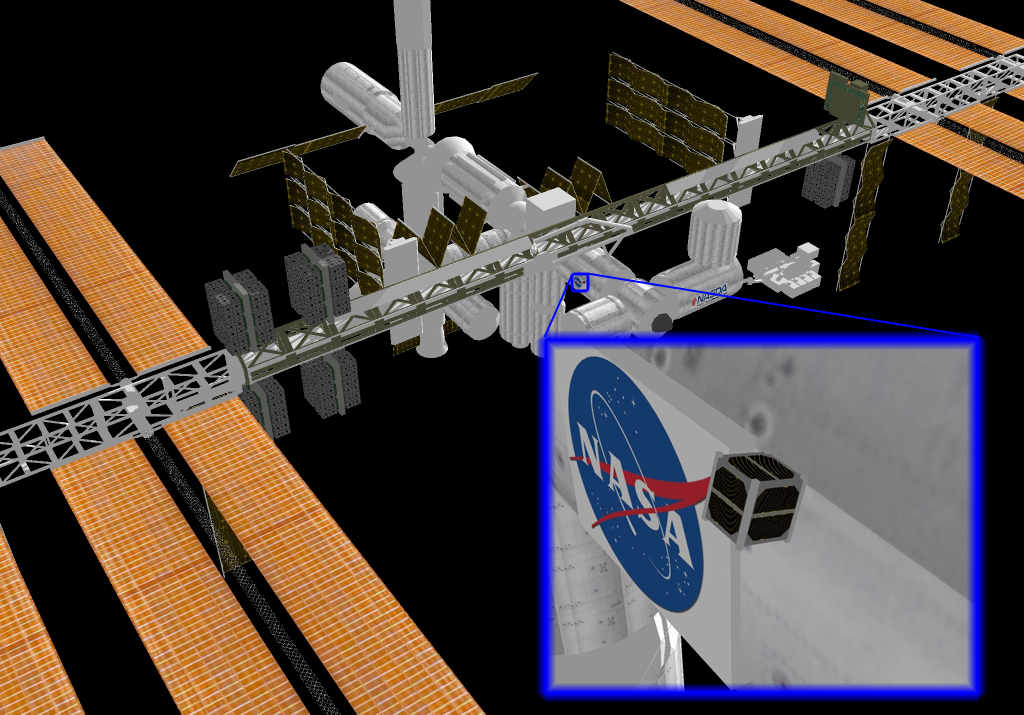
\includegraphics[width = 6cm, height = 6cm ]{figures/iss_inspector.jpg}
\caption{A chaser traverses the surface of the ISS using induction couplers}
\label{fig:iss_inspector}
\end{figure}

\section{Induction Coupler Behaviors}
\label{sec:behavior}
\subsection{Simplified Model}
\label{sec:simple_model}
Of particular interest for the case of planar motion are induction couplers that include permanent magnets. Such an induction coupler consists of a mechanism that spins one or more permanent magnets at a variable speed. In its most elementary form, a permanent-magnet induction coupler uses only a single dipole that spins in a plane. However, each mechanism within the induction coupler can include any number of magnets. A large $\vert \textbf{B} \vert$ and $\nabla \textbf{B}$ maximizes the eddy-current force produced by the array of magnets. These properties can be achieved by using any number of dipoles orthogonal to the spin axis, or a circular Halbach array consisting of dipoles alternating between perpendicular and parallel to the spin axis.

\begin{figure}
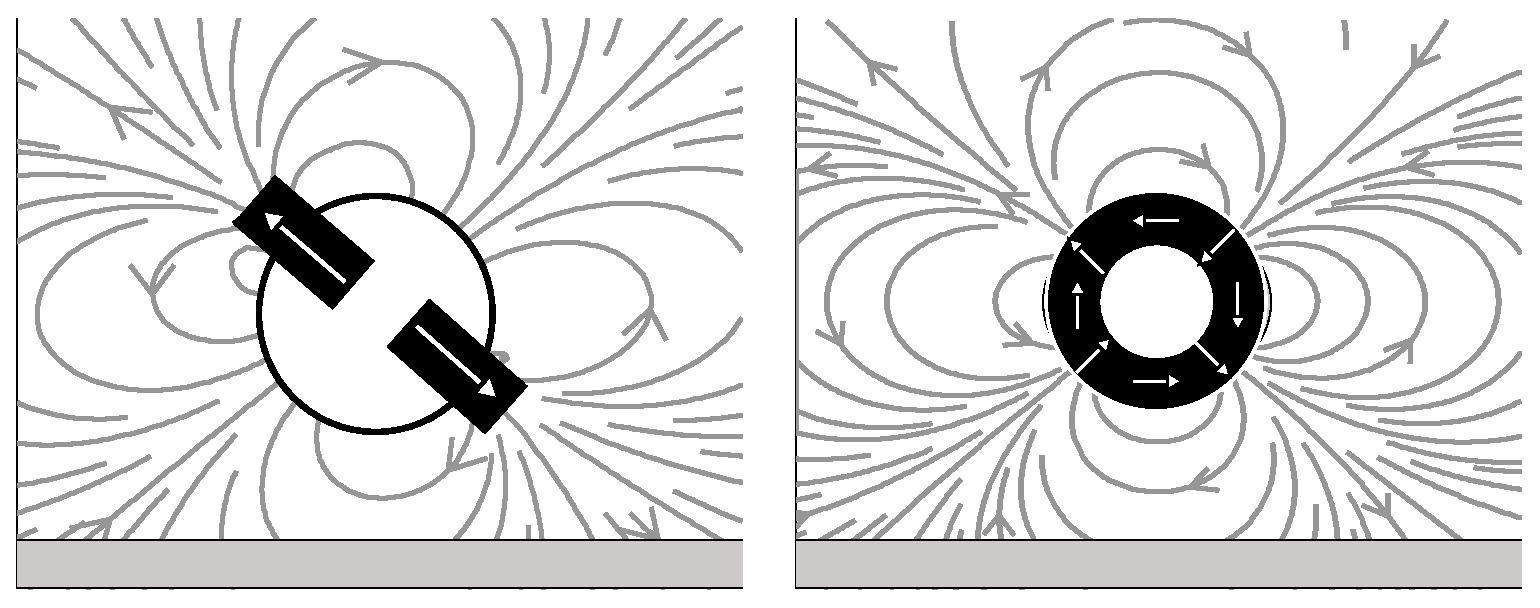
\includegraphics[width = 6cm, height = 6cm ]{figures/two_different_arrays.eps}

\caption{Two different magnet arrays with their magnetic fields and dipole moments near a plate. The field two-magnet orthogonal array is similar to a two pole-pair Halbach array(right.) Each generates force by spinning about an axis out of the page. An orthogonal array is easier to build and the forces from a Halbach array are easier to model.  }
\label{fig:magnet_arrays}
\end{figure}

The more magnets in an array, the more uniform the magnetic field becomes, smoothing the spatial variation in the magnetic field that the target sees. This smoothness decreases the change in the magnetic field as the magnets spin, which may be undesirable in an application that requires high eddy-current force. The number of magnets per array is one of the many considerations in the design of an induction coupler.

A straightforward example of an induction-coupler system is a single array spinning about an axis $\hat{\boldsymbol{a}}$ near conductive surface with a normal vector $\hat{\boldsymbol{n}}$. In this example, the force is 
\begin{equation}\label{eq:singlemagforce}
\textbf{F} = C\left[  \left(1-\beta \right )\hat{\boldsymbol{a}}{\times}\hat{\boldsymbol{n}} + \beta\hat{\boldsymbol{n}} \right ] \omega
\end{equation}

The factor $C$ scales spin speed of specific magnet arrays to the magnitude of the force they produce. $C$ is a function of the magnet properties, target properties, and $\boldsymbol{x}$. $\beta$ is the thrust ratio between the components of the force perpendicular and tangent to the target's surface. $\beta$ changes nonlinearly with $\omega$ and the array's relative speed to the surface, but for small $\omega$, $\beta$ approximately zero so the force is approximately tangential to the surface. 

This model of the force makes two simplifying assumptions based on the planar inspection use case:
\begin{itemize}
\item{Assumption 1:} The angular speed and translational speed of the coupler are both small. At low speeds, the relationship between \textbf{F} and $\omega$ is approximately linear. This linearity is present in the nonlinear model (fig. \ref{fig:lin_fit}) and experimental data (fig. \ref{fig:force_plot}.)
\item{Assumption 2:} The array's axis remains perpendicular to the plate.  

\end{itemize}


\begin{figure}
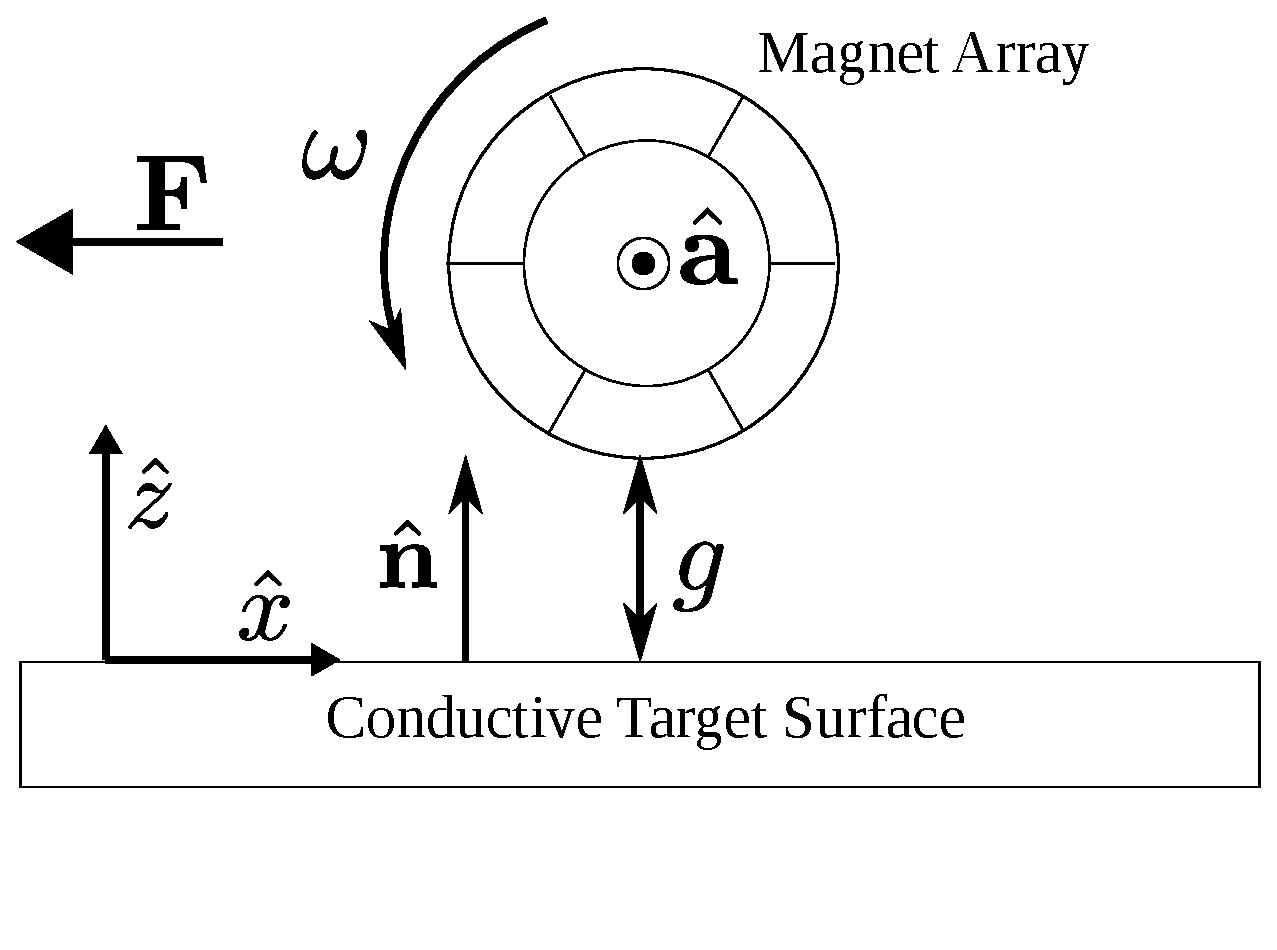
\includegraphics[width = 6cm, height = 6cm ]{figures/spin_mag_diagram.eps}

\caption{A dipole spinning with positive ($\omega$) about its axis $\hat{\textbf{a}}$ at distance g above a target that extends out of the page generates a force \textbf{F} directed to the left.}
\label{fig:arry_force_diagram}
\end{figure}

During in-plane movement, each array is associated with a single control degree of freedom. Its force and torque may project onto any of the six rigid-body degrees of freedom, depending upon geometries: the orientation of the coupler relative to the spacecraft's center of mass, distance between the coupler and the surface, and the topography of the surface. To first order, for a flat plate and a spin axis in a plane perpendicular to the surface normal, the effect is a force only, with no significant moment. The chaser spacecraft can use this force to torque itself if is the force acts at a moment arm relative to the chaser's center of mass. Alternatively, two couplers can create a moment through a couple, which is be independent of the coupler's position relative to the target's mass center.

%% BEN I THINK THIS FIGURE IS UNCESSARY
\begin{figure}
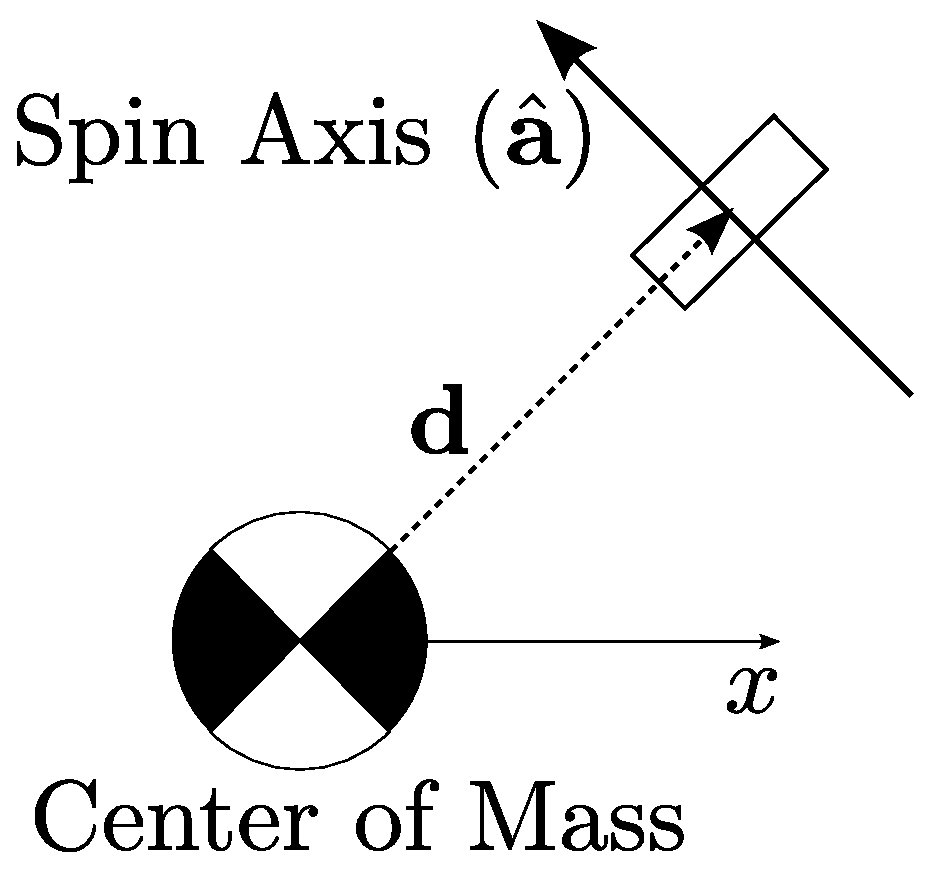
\includegraphics[width = 6cm, height = 6cm ]{figures/simple_geometry.eps}

\caption{A single-magnet induction coupler.}
\label{fig:min_array_diagram}
\end{figure}

\begin{figure}
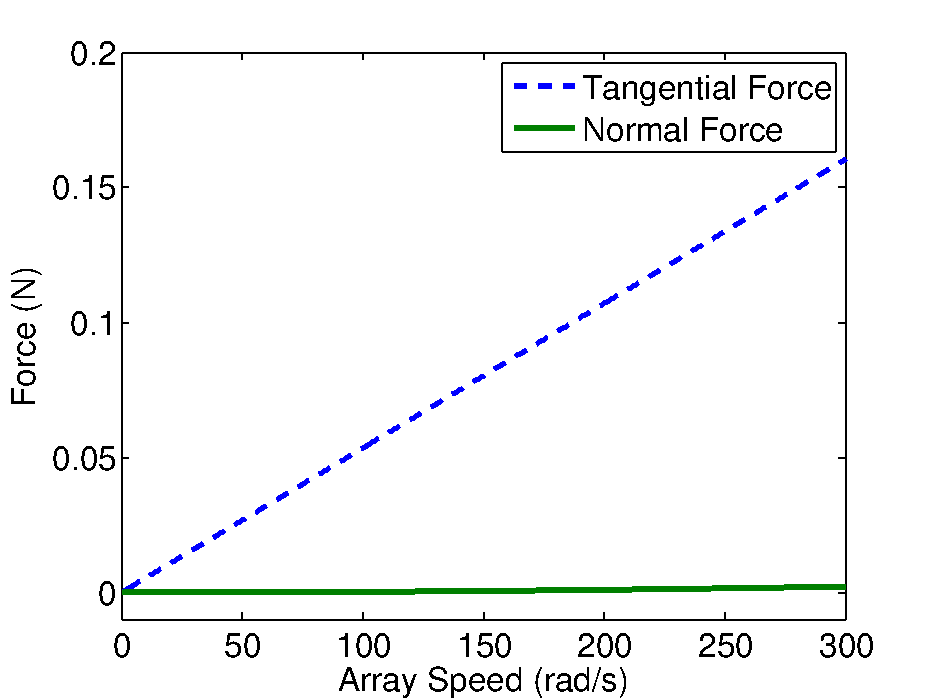
\includegraphics[width = 6cm, height = 6cm ]{figures/tan_v_norm_force.pdf}

\caption{Shear and normal forces on the induction coupler under nominal operating conditions}
\label{fig:tan_v_norm_f}
\end{figure}

\subsection{Induction Coupler Experiments}
\label{sec:experiment}
Experimental development of an induction coupler verifies models showing that this force varies with the magnitude and sign of $\omega$ and demonstrates that the couplers can produce milliNewton shear forces perpendicular to a surface for low power. Figure \ref{fig:force_plot} shows the input-output relationship between the motor speeds and the eddy-current forces they produce. In the demonstrations described here, force is achieved using two small COTS motors (BaneBots MP-36004-540) and neodymium magnets. Figure \ref{fig:cart_picture} shows the experiment  and table \ref{tab:exp_vals} shows the parameters used in the experiment.

\begin{table}
\caption{\label{tab:exp_vals} Experiment Values}
\begin{ruledtabular}
\begin{tabular}{ccc}
Variable & Value & Unit \\
\hline
 Motor Voltage & 12 & V\\
 Duty Cycle & 25 & \%max\\
 Motor Speed & 4200 & RPM \\
 Motor Current & 0.25 & A \\
 Motor Power & 0.75 & W \\
\end{tabular}
\end{ruledtabular}
\end{table}

\begin{table}
\caption{\label{tab:eforce_comparison} Specific Force Comparison}
\begin{ruledtabular}
\begin{tabular}{cc}
System & Specific Force (mN/W) \\
\hline
 Induction Couplers & 3.33 \\
 Electromagnetic Dipoles & 1.22 \cite{Kong2004} \\
 Coulomb Interactions & 3*$10^{-7}$ \cite{king2002spacecraft}\\
\end{tabular}
\end{ruledtabular}
\end{table}

\begin{figure}
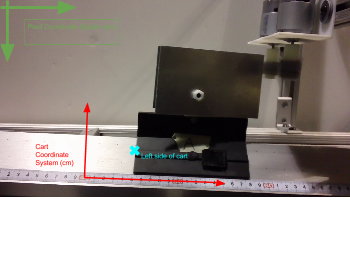
\includegraphics[width = 6cm, height = 6cm ]{figures/cart_on_track.png}

\caption{An aluminum target on a low-friction air track (left) is moved by two spinning magnets (upper right.)}
\label{fig:cart_picture}
\end{figure}


\begin{figure}
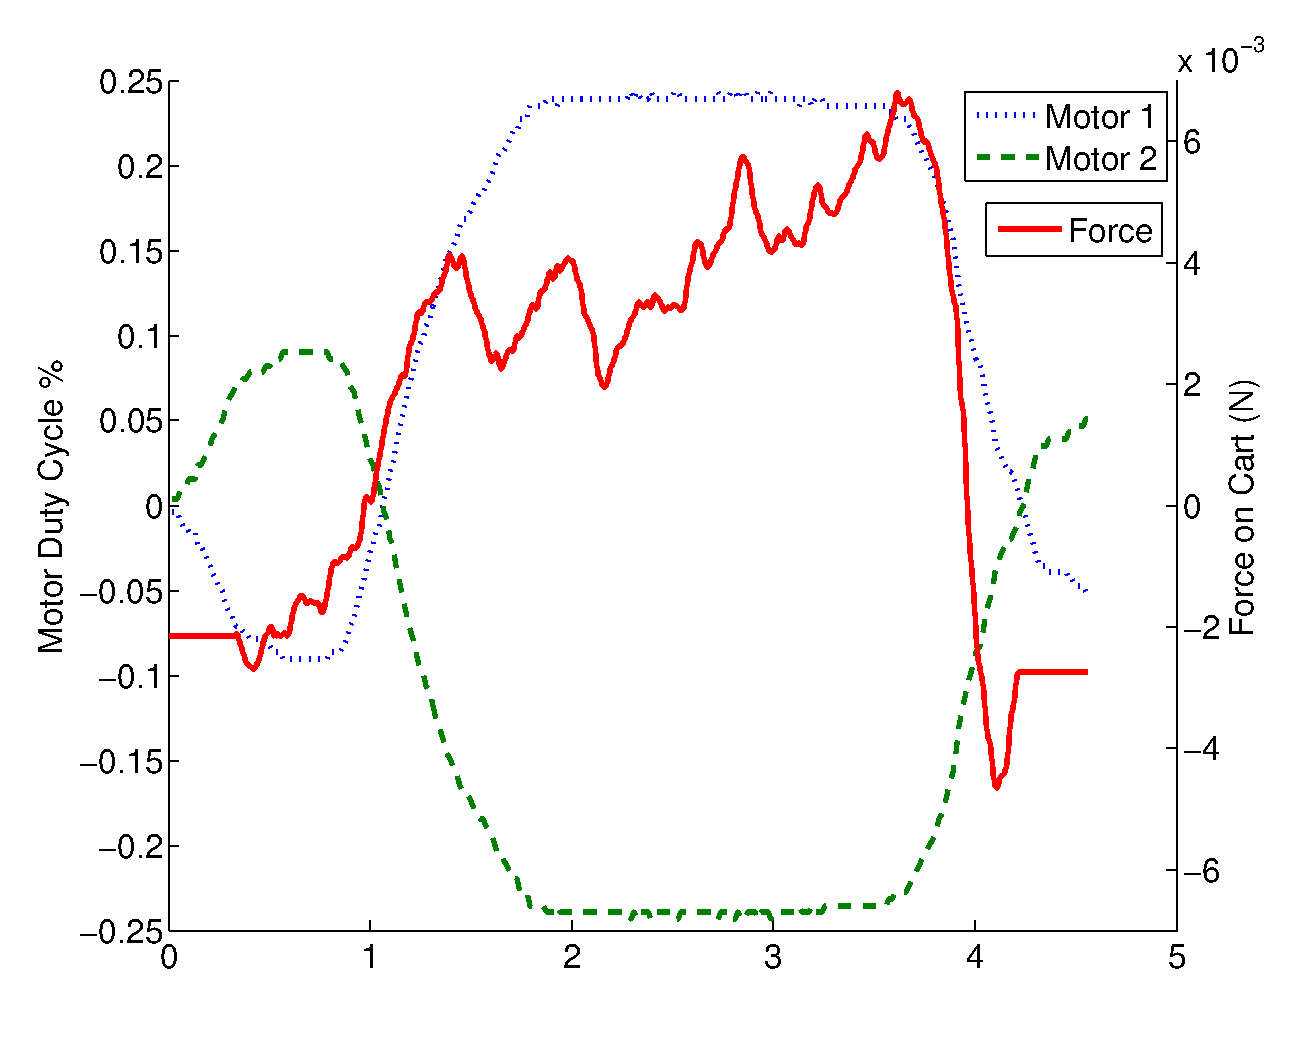
\includegraphics[width = 6cm, height = 6cm ]{figures/motor_force_speed_plot.pdf}

\caption{Force on a one-dimensional air-track levitated cart vs. motor speed for a small, two-motor induction coupler. Oscillations in the force reported here are due to a combination of sensor artifacts and the dynamics of the cart.}
\label{fig:force_plot}
\end{figure}

The steady-state model of eddy-current forces makes two assumptions: that $\frac{1}{\omega}$ is much larger than the characteristic time of the LR circuit approximated by the bulk conductor and that the kinematics of the chaser and target are much slower than the period of rotation of the spinning magnetic fields that act on the target.

There are many other parameters governing induction-coupler force that any implementation of the system needs to consider. The force magnitude decreases with $\frac{1}{g^4}$. Larger magnets provide stronger fields that increase the force. Greater thickness and 
conductivity of the target increase the induced current and thereby scale up the force. Spin speed increases the force nonlinearly by increasing the rate of change in the magnetic field. At low speeds this relationship is approximately linear (see fig. \ref{fig:lin_fit}) but increasing speed past a certain point shows diminishing returns because the penetration depth (or skin depth) of the induced current decreases at high frequencies. \cite{Paudel2013} The high dimensionality of this system motivates future work to algorithmically find suitable induction coupler design for different applications.

\section{The Induction Coupler System}

The rotational speed of each array controls the force between that array and the surface of the target. The sum of the forces from all the arrays and their resultant torque can be mapped through the linearized dynamics of the target and chaser to plan control inputs based on a desired maneuver. Nonlinearities are likely best accommodated through gain scheduling, a topic that the authors intend to take up as future work.

With an operating range of a few centimeters, the surface for most of the ISS looks like an infinite plane to the inspection spacecraft. This analysis assumes that the proposed inspection vehicle conforms to the CubeSat standard so the mass of the entire system is not above m = 4 kg.
It is possible for an induction coupler with only one or two spinning arrays to achieve planar motion. That motion is nonholonomic; i.e. the chaser's ability to move in a given direction depends on its orientation.

Three spinning arrays can govern three independent planar degrees of freedom. In practice, more should be used for redundancy and greater control authority. As long as the arrays have sufficient spatial separation their forces simply superimpose without the nonlinear coupling that might arise if one array's induced currents interact with another's magnetic field. A separation of 5.5 times the distance to the surface is enough to cause the magnetic field from one coupler to drop by an order of magnitude in the eddy-current region of the other. For a particular application, these principles inform tradeoffs among force, power, mass, and the reliability of moving parts introduced by the additional arrays.

In the induction coupler, each array is the located on a vector $\boldsymbol{d}$, relative to the spacecraft's center of mass. Each array has a spin axis $\hat{\boldsymbol{a}}$. See \ref{fig:min_array_diagram} The force generated by each array varies linearly with with its angular speed $\omega_i$.

\begin{figure}
\label{fig:lin_fit}
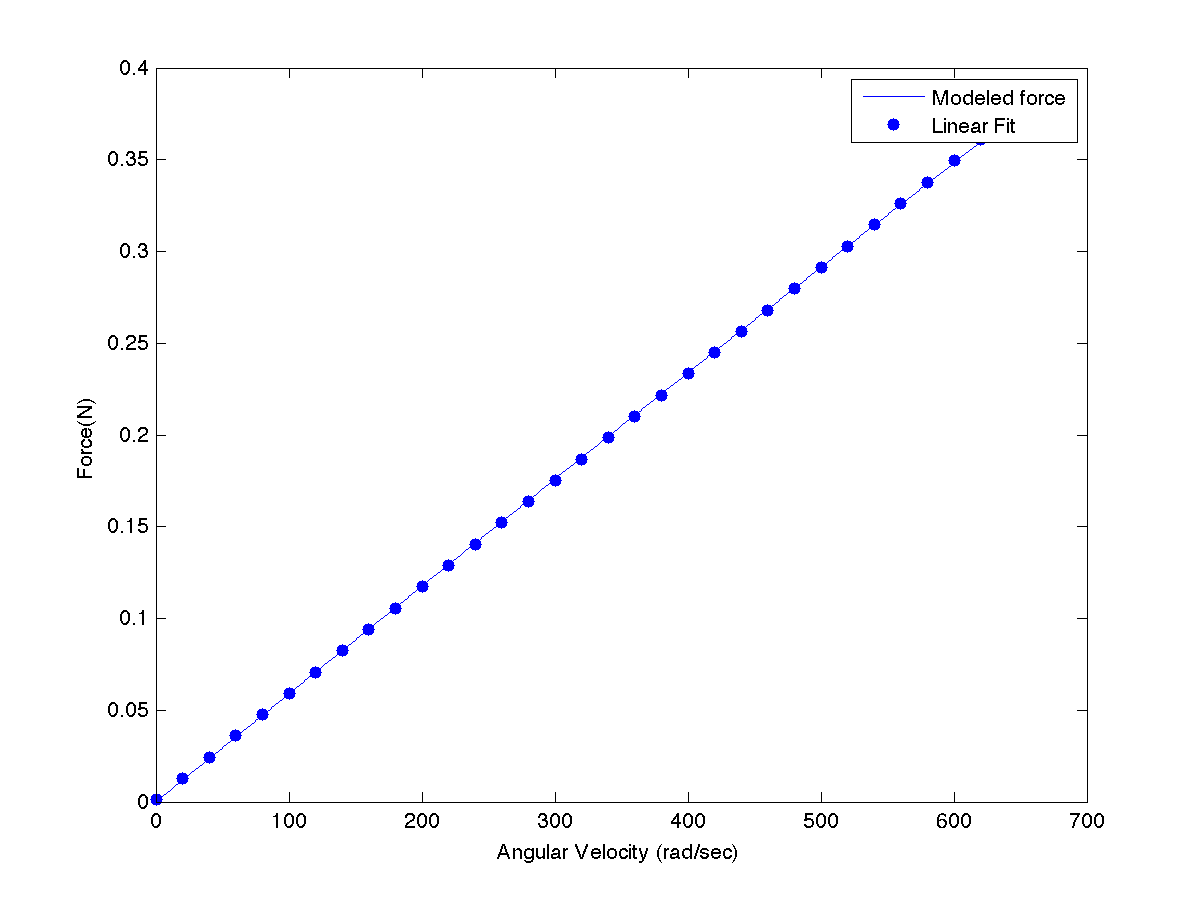
\includegraphics[width = 4cm, height = 4cm ]{figures/lin_fit.png}
\caption{Linear fit between shear force and a magnet array's angular velocity. For the values listed in table \ref{table:values}, the slope is $c = 5.031 * 10^{-4} \frac{N}{rad/s}$}
\end{figure}

%% TODO MASON EDIT
%%I have several questions about notation that arise in this section.  Matrices and scalars should be non-bold.  Vectors and tensors should be boldface.  You should not multiply a matrix by a vector or a tensor.  The superscript X notation is used only for matrices (e.g. 3x1 columns of numbers), which would be non-boldface.

%% TODO MASON EDIT
%% This is fine; make all appearances of 6Dof or 6DOF or 6 DoF consistent.
The system kinematics are those of a standard 6 DoF rigid body. 
\begin{equation}\label{eq:rotMrxPropigation}
\dot{A} = \omega^{\times}A
\end{equation}
\begin{equation}\label{eq:RigidBodyKinematics}
\begin{pmatrix} 
I =\dot{\omega} \\
m\ddot{x}
 \end{pmatrix}
=
\begin{pmatrix} 
-\omega^{ \times} \left( I\omega \right) \\
0
\end{pmatrix}
+
\begin{bmatrix}
1 & 0 \\
0 & A
\end{bmatrix}
Ju
\end{equation}
where A is the direction-cosine matrix that relates the target coordinate system and the chaser coordinate system. Here, $\omega$ and $x$ are the chaser's angular velocity and position. Note that the chaser angular velocity ($\omega$) is separate from the input speed of coupler i ($\omega_i$.)  $I$ is the chaser's inertia tensor and $m$ is its mass.
\begin{equation}
\label{eq:u_definition}
u = 
\begin{bmatrix}
\omega_1\\
\omega_2\\
...\\
\omega_N
\end{bmatrix}
\end{equation}
The control input $u$ is a column matrix of N speed commands - one for each coupler.

\begin{equation}\label{eq:Jacobian}
J = C\begin{bmatrix} 
d_1^{\times}\left[ \left(1-\beta_1 \right )\hat{a}_1^{\times}\hat{n} + \beta_1\hat{n}\right ]&
d_2^{\times}\left[\left(1-\beta_2 \right )\hat{a}_2^{\times}\hat{n} + \beta_2\hat{n}\right ] &
 ... &
d_N^{\times} \left[\left(1-\beta_N \right )\hat{a}_N^{\times}\hat{n} + \beta_N\hat{n}\right ]
\\

\left(1-\beta_1 \right )\hat{a}_1^{\times}\hat{n} + \beta_1\hat{n}&
\left(1-\beta_2 \right )\hat{a}_2^{\times}\hat{n} + \beta_2\hat{n} &
 ... &
 \left(1-\beta_N \right )\hat{a}_N^{\times}\hat{n} + \beta_N\hat{n}
\end{bmatrix}
\end{equation}
The Jacobian \ref{eq:Jacobian}  imposes constraints on the design of the induction coupler and the chaser's mission.

\begin{itemize}
\item  $\boldsymbol{d}_i{\times}\hat{\boldsymbol{a}}_i$ must be nonzero for at least one array, corresponding to the requirement that all of the spin axes cannot be perpendicular to their moment arms, nor can all $\boldsymbol{d}_i$ be zero (i.e. some of the arrays cannot be at the unlikely location of the target spacecraft's center of mass).
\item  Not all of the spin axes $\hat{\boldsymbol{a}}_i$ can be parallel. If they were, the Jacobian would not be full rank.
\end{itemize}

An induction coupler of this type on a 4 kg spherical spacecraft of radius 0.1 m, can generate a linear acceleration of
$a = 2*10^{-3} \frac{m}{s^2}$ 
and an angular acceleration of 
$\alpha = 9*10^{-3} \frac{rad}{s^2}$. 
These values, while modest, allow an inspection vehicle to overcome typical LEO perturbation forces
\cite{wertz2011space}
 and move slowly over the surface of the ISS to inspect it. These values are based on the small prototype comprised of COTS components and an induction coupler as described above, with only three magnet arrays. Using additional arrays and using more efficient hardware like high-speed brushless motors are two straightforward ways to increase the capabilities in this example.

A three-array inspection spacecraft performing a maneuver near a flat surface illustrates the capabilities of the induction-coupler system. 

The present analysis assumes that the inspection spacecraft maintains a small constant distance from the surface. The analysis assumes that the force normal to the surface can be ignored, so all motion remains in the plane parallel to the surface. 

The results from a simulation of an inspection vehicle in figures \ref{fig:trajectory} and \ref{fig:theta_and_speeds} with the parameters in table \ref{table:values} demonstrates that a small spacecraft can use induction couplers and PD control to inspect a large area in a 
reasonable amount of time. With a 0.1 m inspection swath, it could cover the 39 $m^2$ surface of the Destiny ISS module in just under two hours.   

\begin{figure}

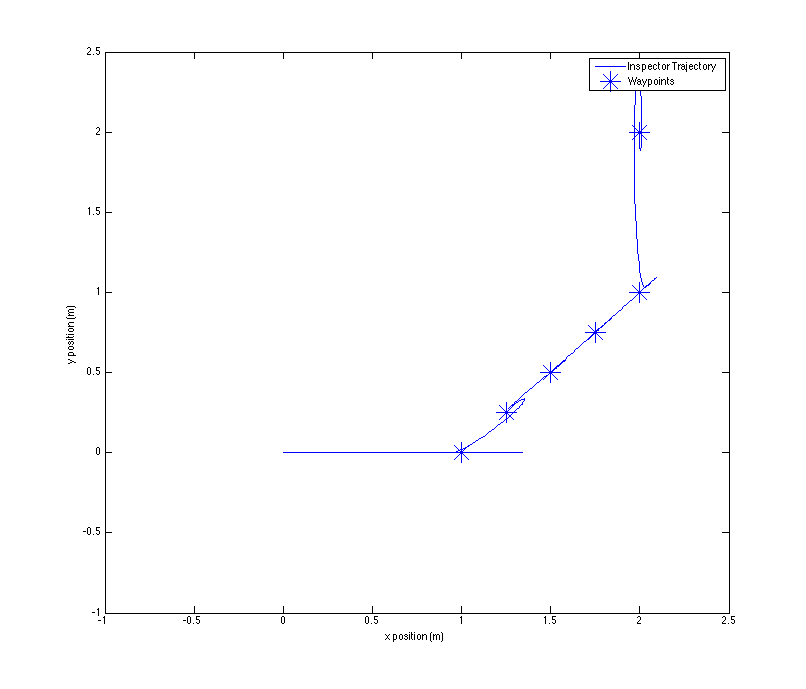
\includegraphics[width = 6cm, height = 6cm ]{figures/planar_trajectory.png}
\caption{Trajectory of a simulated inspection vehicle. Using conservative parameters A series of waypoints specify a path 3.4 m long with a 90 degree turn. }
\label{fig:trajectory}
\end{figure}

\begin{figure}

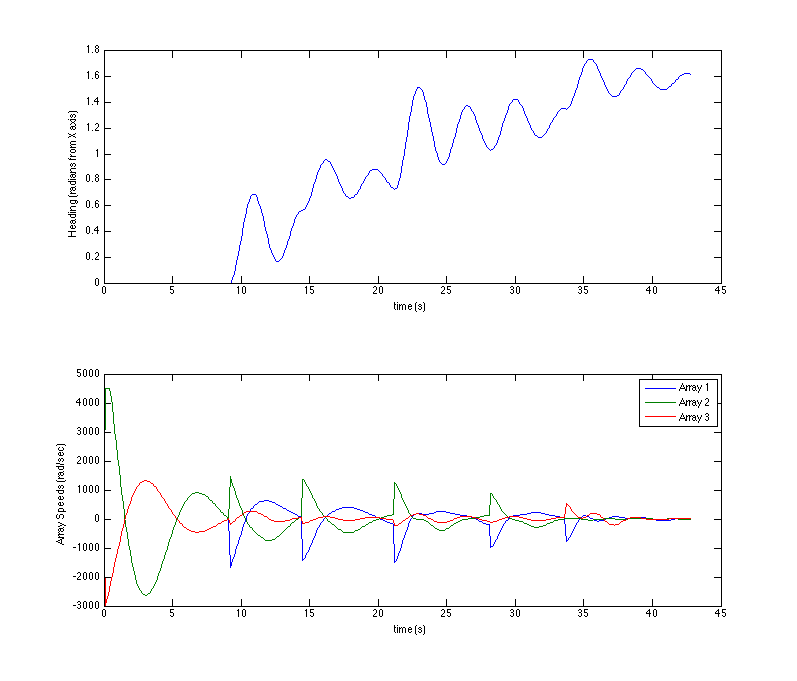
\includegraphics[width = 6cm, height = 6cm ]{figures/theta_and_speed.png}
\caption{Heading and speed for a simulated inspection vehicle. }
\label{fig:theta_and_speeds}
\end{figure}



\begin{table}[ht]
\caption{Model Values} % title of Table
\centering % used for centering table
\begin{tabular}{c c c} % centered columns (4 columns)
\hline\hline %inserts double horizontal lines
Variable & Value & Units\\ [0.5ex] % inserts table 
\hline
%heading

$r_i$ & 0.0127 & m\\  
$r_o$ & 0.0191 & m \\
$B_r$ & 1.42 & T \\
$\mu$ & 1.08 & \\
g & 0.01 & m\\

$\sigma$ & $3.53 * 10^5$ & $\frac{S}{m}$ \\
b & 0.01 & m\\
$m$ & 4 & kg \\
$I$ & 0.16 & kg$m^2$

 \\ [1ex] % [1ex] adds vertical space
\hline %inserts single line
\end{tabular}
\label{table:values} % is used to refer this table in the text
\end{table}


\begin{figure}
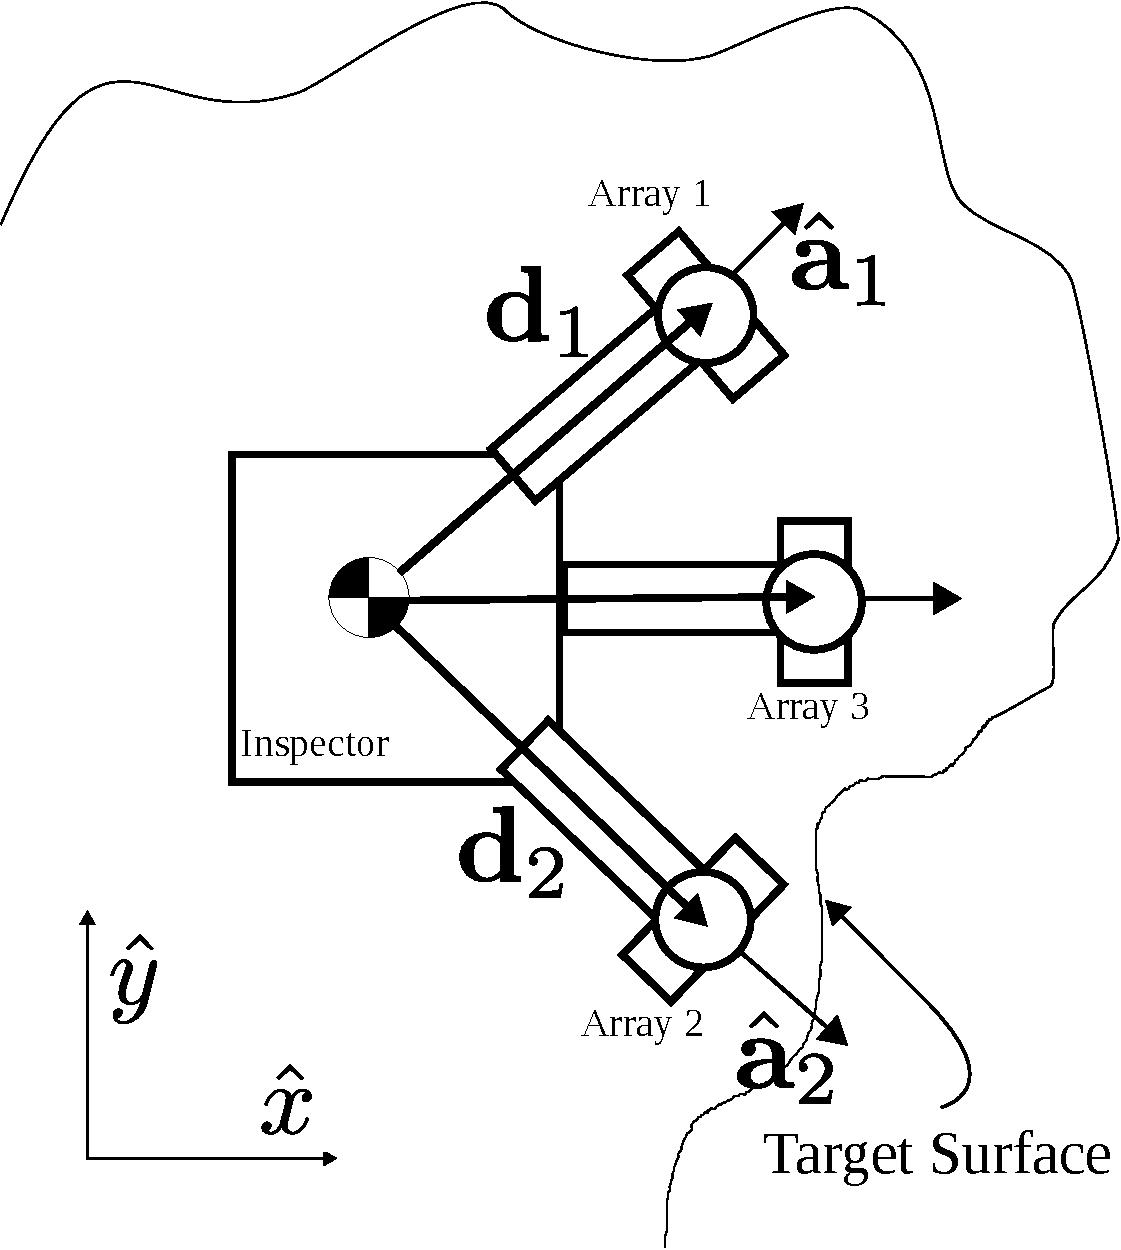
\includegraphics[width = 6cm, height = 6cm ]{figures/surface_locomotion-eps-converted-to.pdf}
\label{fig:sample_coupler}
\caption{Example induction coupler architecture with three single-magnet arrays.}
\end{figure}
\section{Conclusion}
This paper presents a starting point for induction coupler technology. It describes the physics of spinning magnet arrays that produce contactless force and torque on any conductive target. Preliminary experiments verified and measured these forces, which are both larger and less power-hungry than other contactless actuators. Simulations have demonstrated how the force can be used to maneuver an inspection vehicle. 

Induction couplers offer the prospect of inter-body force that enables close-proximity inspection of a larger target vehicle by a smaller chaser spacecraft, all without mechanical contact. There are many paths for future induction coupler research that extends this key conclusion. This analysis included only planar motion. Future work will explore full six-degree-of-freedom maneuverability.
%% TODO compare forces to other technology
\section*{Acknowledgments}
This work was supported by NASA NSTRF Grant \#NNX11AN46H %TODO PUT NUMBER HERE
\section*{References}
\bibliographystyle{plain}
\bibliography{biblio.bib}
\end{document}


[1]Why is this repeated whole cloth from the abstract?
[2]I'm not sure that this sentence belongs in this paragraph, but in any case it can't serve as its own paragraph.  Go for at least 3 sentences per paragraph.
[3]Need a transition sentence at the beginning of this paragraph.
[4] This paragraph is not true and needs to be changed iin a way that isn’t comp
[5]This sentence is meant to serve as a conclusion.  The paragraph needs one.  If you don't like this one, write another.
[6]Cite one of the hundreds of papers describing this "non-destructive evaluation" technique.
[7]I moved these two sentences here because they makes more sense in the flow of the paragraph, but now it seems redundant.  Get rid of it?
[8]Deleted because it seems redundant.
[9]replace "small" with a model number and manufacturer
[10]Format correctly
[11]Can you compare this value of mN/W to the force/power for typical ion propulsion, EMFF, and Coulomb approaches offer?  Do so in the conclusion, not here.
[12]Do you have citations for these principles and/or some specific dependencies (linear, etc?)
[13]These two sentences are not connected to the text around them.  Do they belong here?  I have no problem with what’s being said, but why is it being said here?  What larger point is being made?
[14]I have several questions about notation that arise in this section.  Matrices and scalars should be non-bold.  Vectors and tensors should be boldface.  You should not multiply a matrix by a vector or a tensor.  The superscript X notation is used only for matrices (e.g. 3x1 columns of numbers), which would be non-boldface.
[15]This is fine; make all appearances of 6Dof or 6DOF or 6 DoF consistent.
[16]What numbers do you have?
[17]Combine these discrete sentences into a paragraph with an introductory sentence and a conclusion
[18]Here’s where you should compare your experimental results to the scale of forces available from the other technologies, concluding that your concept is not only viable but better in N/W.
